%%%%%%%%%%%%%%%%%%%%%%%%%%%%%%%%%%%%%%%%%
% NIWeek 2014 Poster by T. Reveyrand
% www.microwave.fr
% http://www.microwave.fr/LaTeX.html
% ---------------------------------------
% 
% Original template created by:
% Brian Amberg (baposter@brian-amberg.de)
%
% This template has been downloaded from:
% http://www.LaTeXTemplates.com
%
% License:
% CC BY-NC-SA 3.0 (http://creativecommons.org/licenses/by-nc-sa/3.0/)
%
%%%%%%%%%%%%%%%%%%%%%%%%%%%%%%%%%%%%%%%%%

%----------------------------------------------------------------------------------------
%   PACKAGES AND OTHER DOCUMENT CONFIGURATIONS
%----------------------------------------------------------------------------------------

\documentclass[a0paper,portrait]{baposter}

\usepackage[font=small,labelfont=bf]{caption} % Required for specifying captions to tables and figures
\usepackage{booktabs} % Horizontal rules in tables
\usepackage{relsize} % Used for making text smaller in some places

\usepackage{amsmath,amsfonts,amssymb,amsthm} % Math packages
\usepackage{eqparbox}

\usepackage{textcomp}

\graphicspath{{figures/}} % Directory in which figures are stored

 \definecolor{bordercol}{RGB}{40,40,40} % Border color of content boxes
 \definecolor{headercol1}{RGB}{186,215,230} % Background color for the header in the content boxes (left side)
 \definecolor{headercol2}{RGB}{120,120,120} % Background color for the header in the content boxes (right side)
 \definecolor{headerfontcol}{RGB}{0,0,0} % Text color for the header text in the content boxes
 \definecolor{boxcolor}{RGB}{210,235,250} % Background color for the content in the content boxes


\begin{document}

\background{ % Set the background to an image (background.pdf)
\begin{tikzpicture}[remember picture,overlay]
\draw (current page.north west)+(-2em,2em) node[anchor=north west]
{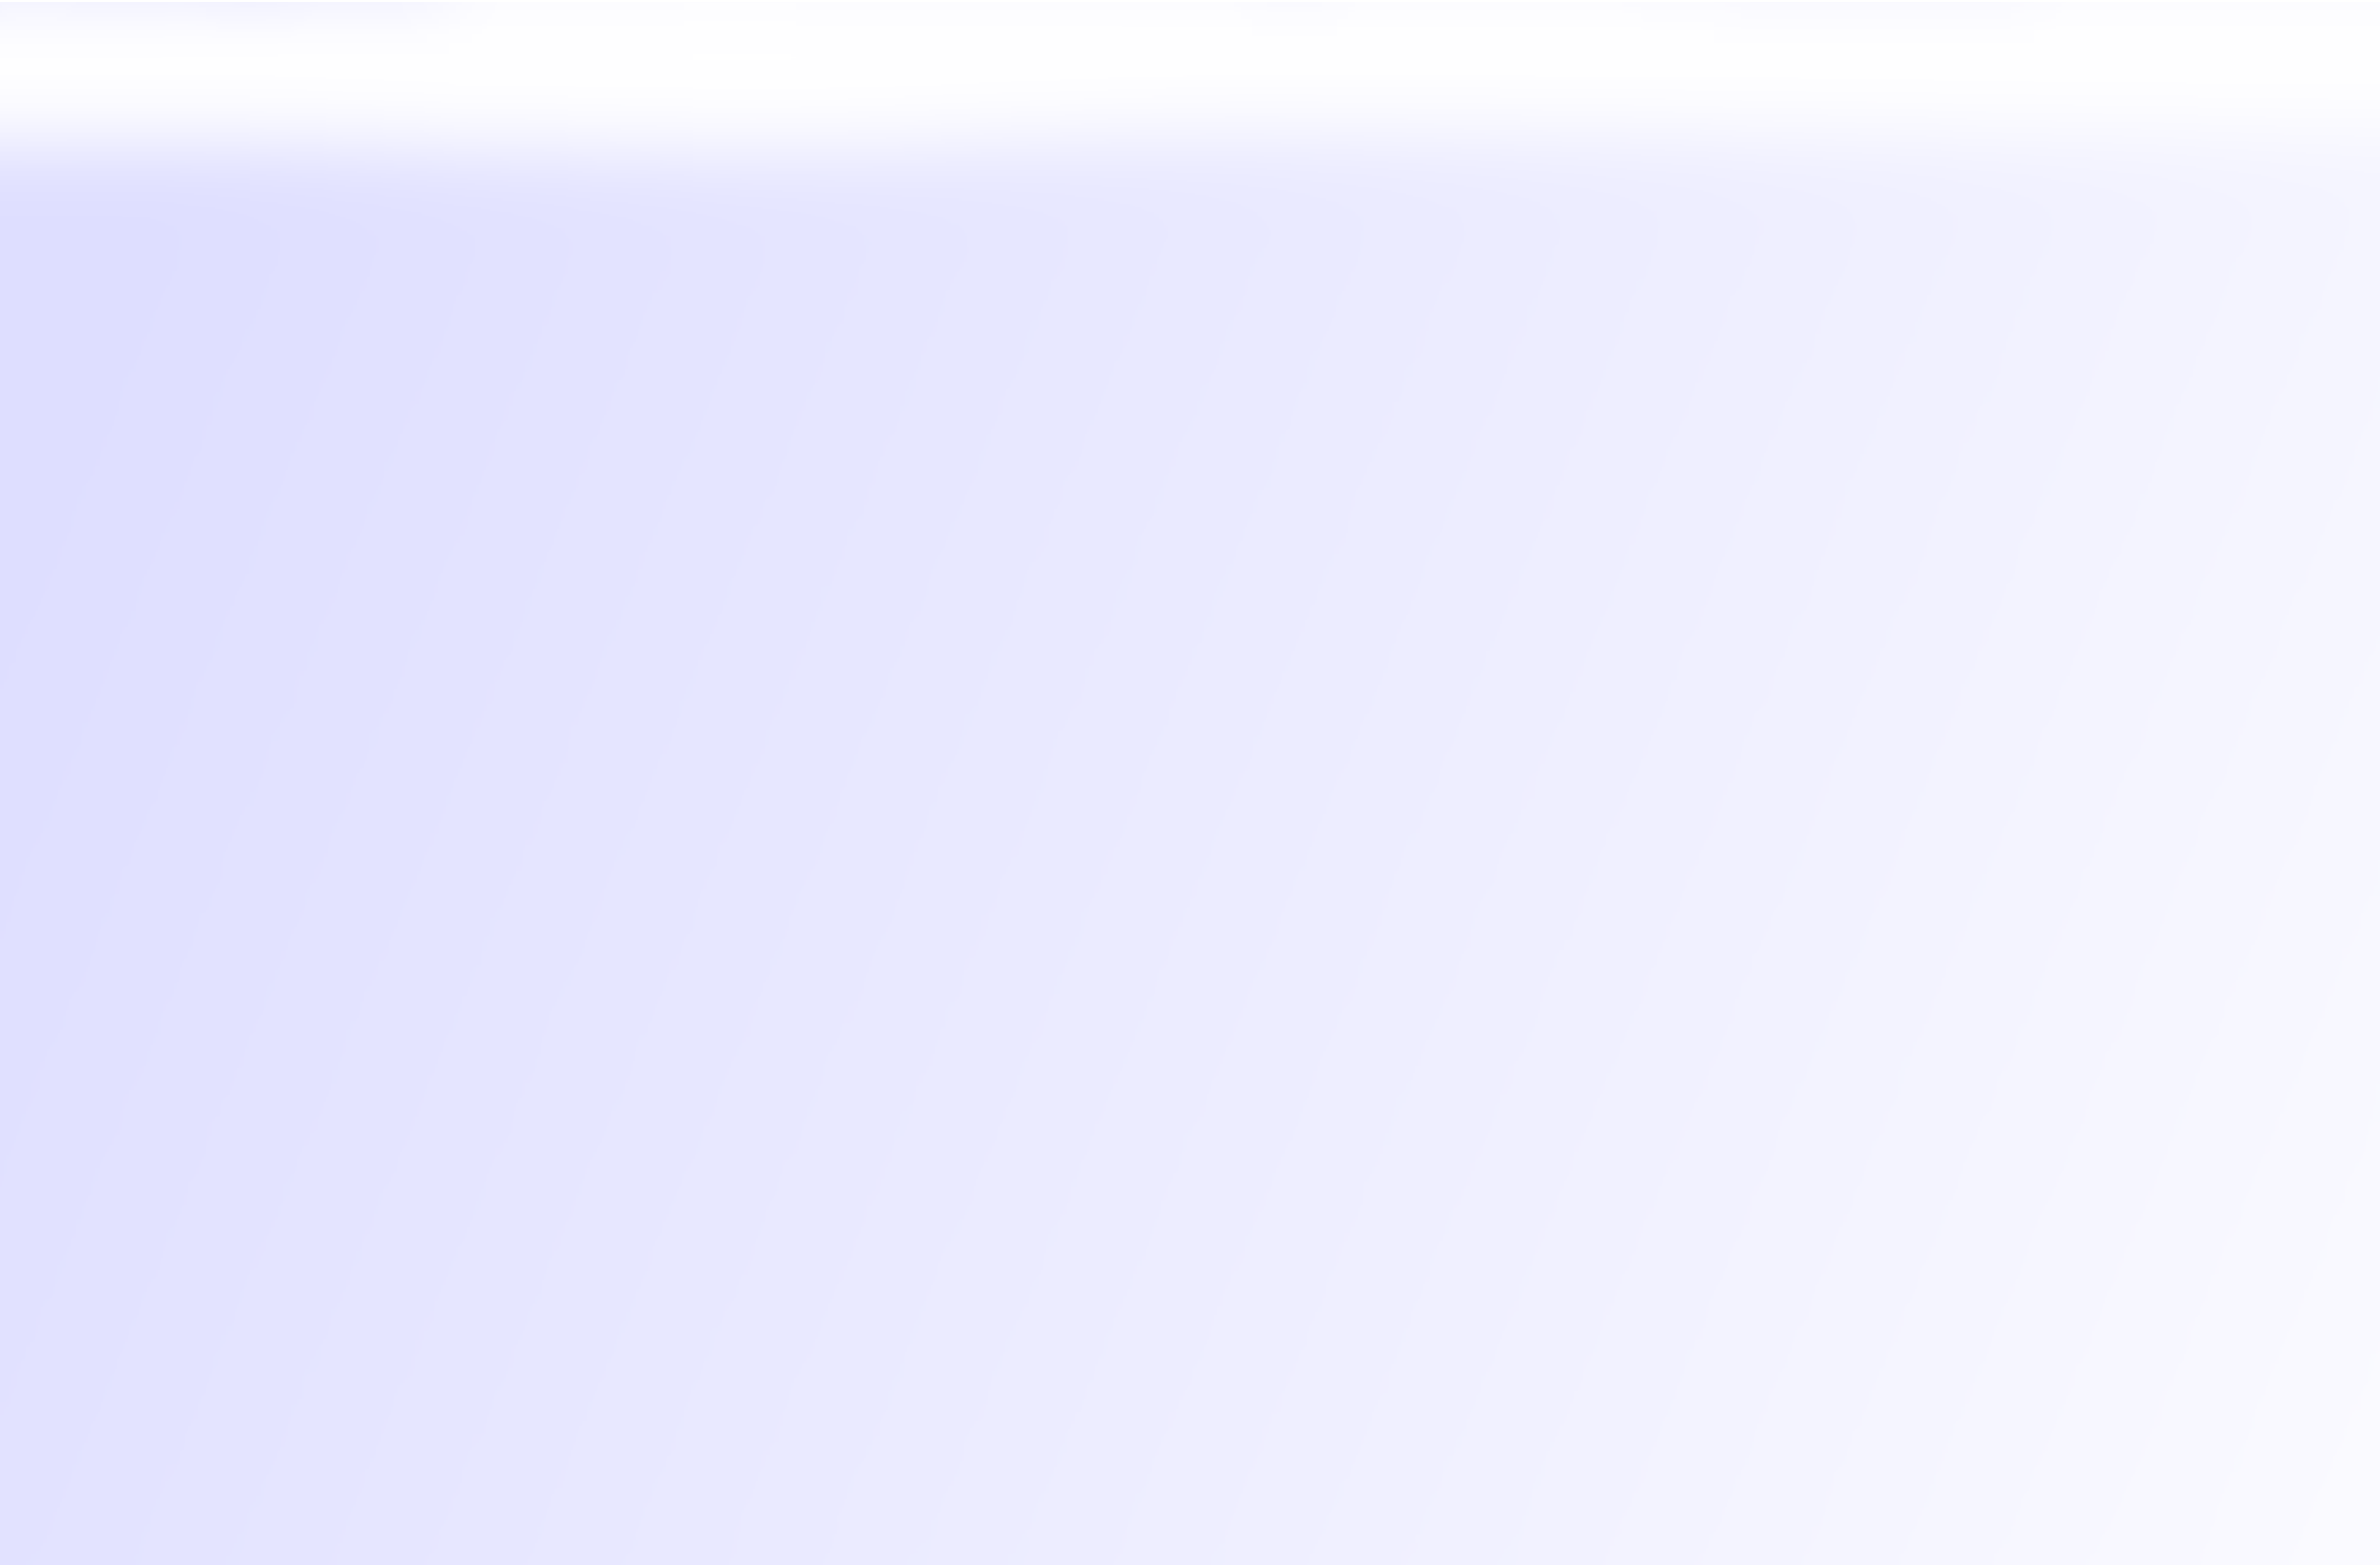
\includegraphics[height=1.1\textheight]{background}};
\end{tikzpicture}
}

\begin{poster}{
grid=false,
columns=4,
borderColor=bordercol, % Border color of content boxes
headerColorOne=headercol1, % Background color for the header in the content boxes (left side)
headerColorTwo=headercol2, % Background color for the header in the content boxes (right side)
headerFontColor=headerfontcol, % Text color for the header text in the content boxes
boxColorOne=boxcolor, % Background color for the content in the content boxes
headershape=roundedright, % Specify the rounded corner in the content box headers
headerfont=\Large\sf\bf, % Font modifiers for the text in the content box headers
textborder=rectangle,
background=none,
headerborder=open, % Change to closed for a line under the content box headers
boxshade=plain
}
{
\includegraphics[scale=0.3]{CU.png}}
%
%----------------------------------------------------------------------------------------
%   TITLE AND AUTHOR NAME
%----------------------------------------------------------------------------------------
%
{ \bf  \huge {Large Signal Network Analyzer} \\  \Large \it An affordable PXI-based microwave non-linear characterization platform} % Poster title
{\vspace{0.3em} \smaller Tibault Reveyrand$^1$, Scott Schafer$^1$, John Boudreaux$^1$, Takao Inoue$^2$, Zoya Popovi\'c$^1$   \\  % Author names
  
\smaller $^1$\it {University of Colorado at Boulder} \\ $^2$\it{National Instruments} } % Author email addresses
{
\includegraphics[scale=0.45]{NI.jpg}} % University/lab logo

%----------------------------------------------------------------------------------------
%   INTRODUCTION
%----------------------------------------------------------------------------------------
\headerbox{Introduction}{name=introduction,column=0,row=0, span=4}{
\begin{itemize} 
\item The goal of this research is to integrate microwave-frequency Large Signal Network Analysis capabilities with commercially available National Instruments' PXI modular instrumentation and LabVIEW environment.
\vspace{-0.2cm}
\item The Microwave Research Group at the University of Colorado has decades of experience in UHF through millimeter-wave transmitters, including recent X-band (10-GHz) MMIC implementations in GaN. Our aim is to extend the frequency range and capabilities of available commercial instrumentation provided by NI.
\vspace{-0.2cm}
\item The proposed instrumentation development will enable new types of measurements such as those required for harmonically-terminated PAs, various transmitter architectures (Doherty, outphasing and supply modulated PAs), as well as microwave transistor rectifiers.  The time-domain characterization is expected to provide dramatic improvement in RF circuit design capabilities.
\end{itemize}
}


\headerbox{Bar-Hillel Theorem}{name=bh,column=0,below=introduction, span=2}{
\begin{itemize} 
\item The goal of this research is to integrate microwave-frequency Large Signal Network Analysis capabilities with commercially available National Instruments' PXI modular instrumentation and LabVIEW environment.
\end{itemize}
}


\headerbox{Generalized LL}{name=gll,column=2,below=introduction, span=2}{
\begin{itemize} 
\item The goal of this research is to integrate microwave-frequency Large Signal Network Analysis capabilities with commercially available National Instruments' PXI modular instrumentation and LabVIEW environment.
\end{itemize}
}

%----------------------------------------------------------------------------------------
%   CALIBRATION
%----------------------------------------------------------------------------------------
\headerbox{Linear input parsing}{name=calibration,column=0,below=gll}{
\begin{itemize}
\item Classical
\item Multilexem
\item Error recovery
\end{itemize}
}

%----------------------------------------------------------------------------------------
%   OTHER INSTRUMENTATION
%----------------------------------------------------------------------------------------
\headerbox{Graph parsing}
{name=instruments,column=1,span=2, below=gll}{ % To reduce this block to 1 column width, remove 'span=2'

Graph DB, metagenomic assemblies etc.
}

\headerbox{CF compression}
{name=cfcompression,column=3,row=1, below=gll}{ % To reduce this block to 1 column width, remove 'span=2'

Compressed data processing
}

%----------------------------------------------------------------------------------------
%   MIXER vs. SAMPLERS
%----------------------------------------------------------------------------------------
\headerbox{Generalized LL generalization}{name=receiver,span=4,column=0,row=1, below=calibration}{
\begin{center}
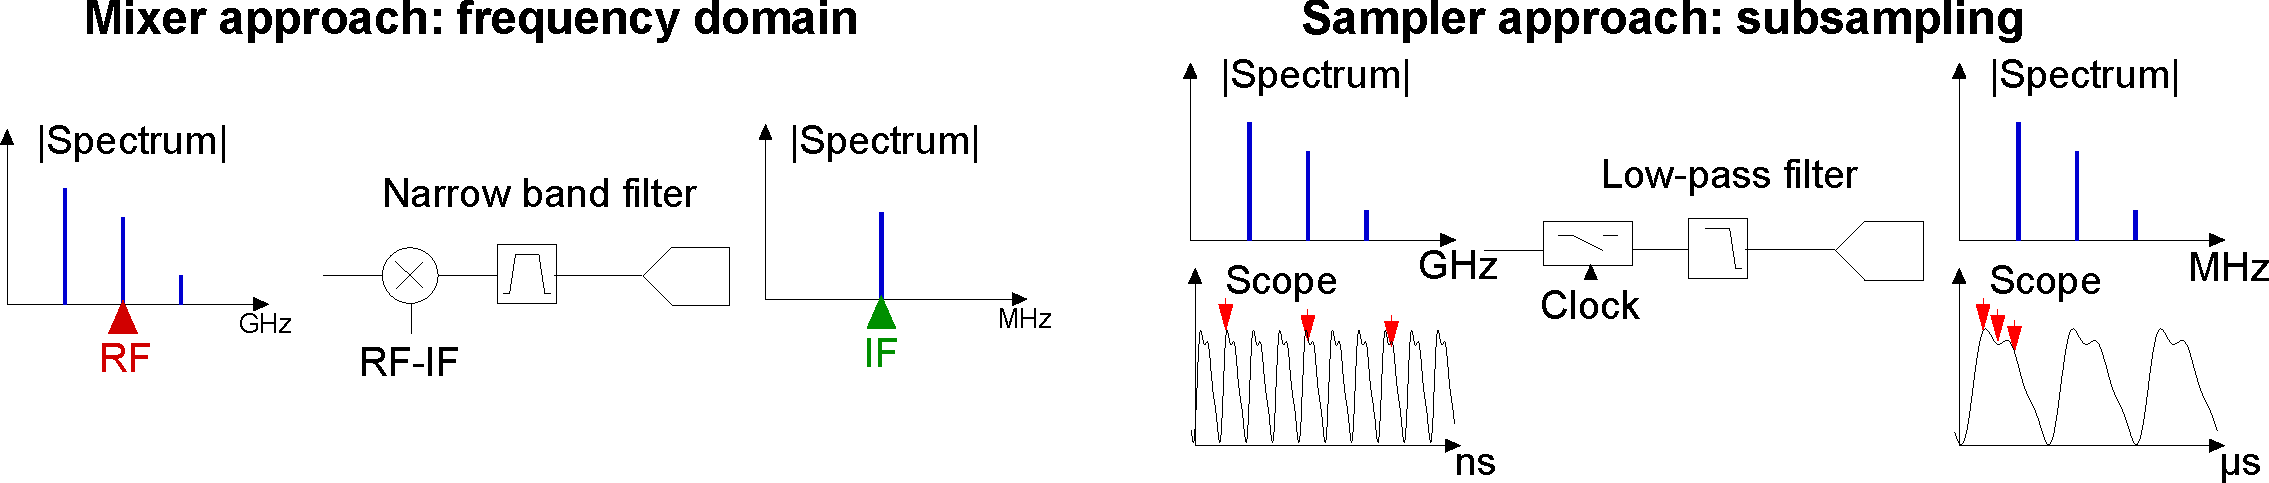
\includegraphics[width=1\linewidth]{RECEIVER.pdf}
\end{center}
}


%----------------------------------------------------------------------------------------
%   MEASUREMENT SETUP
%----------------------------------------------------------------------------------------
\headerbox{Measurement Setup for Envelope Tracking Application}{name=application,span=2,column=1,below=receiver}{ 
The setup includes \textbf{two LSNAs simultaneously}. One is dedicated to RF (sampler based downconversion), the other one samples directly the LF stimulus. The purpose is to investigate \textbf{low-frequencies $S_{22}$} of the DUT under RF large signal conditions.
\begin{center}
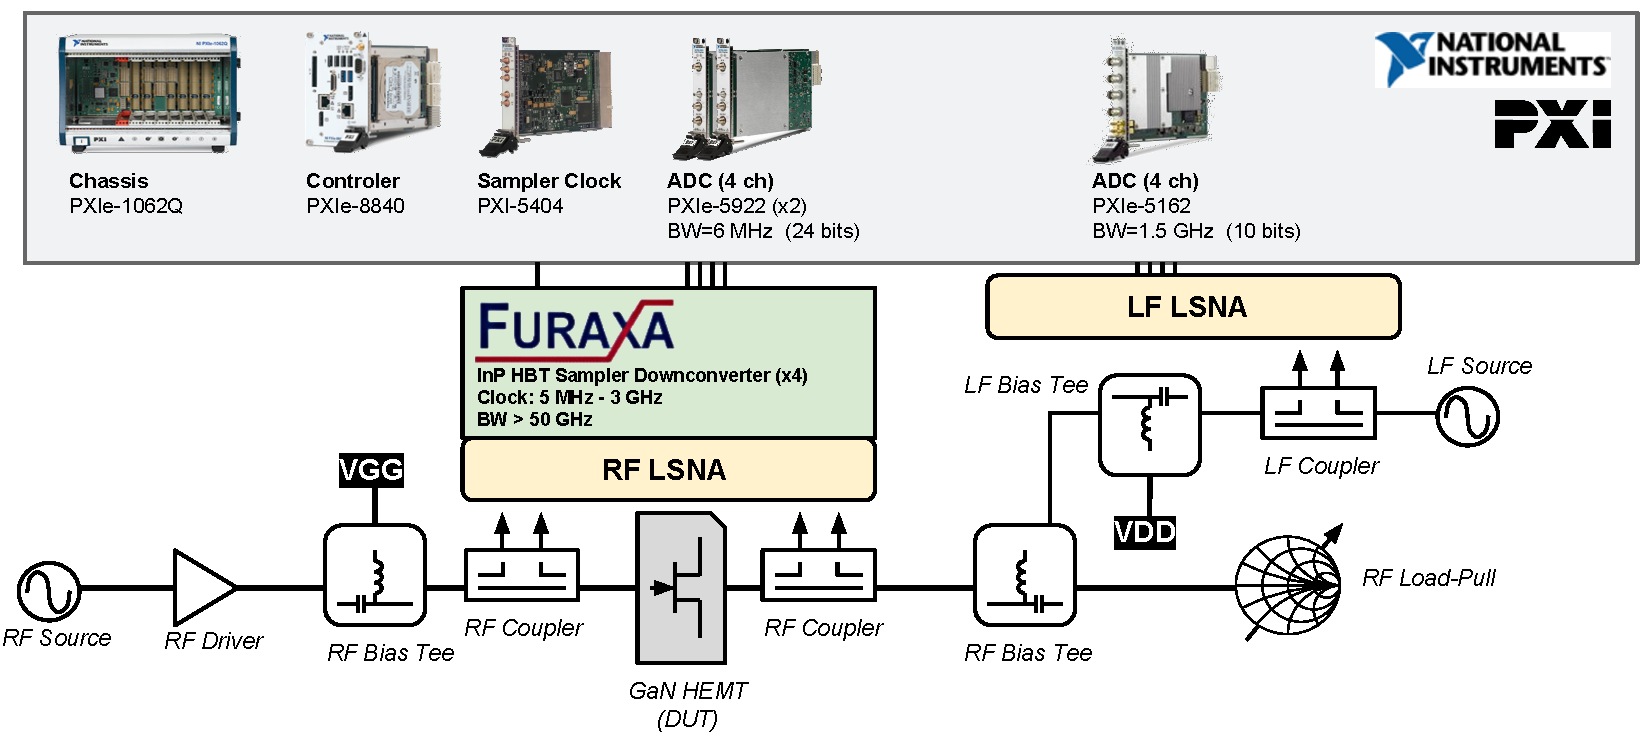
\includegraphics[width=\linewidth]{BENCH.pdf}
\small \textit{Low-frequency measurement of drain supply envelope-bandwidth impedance for supply-modulated PAs}
\end{center}
}


%----------------------------------------------------------------------------------------
%   CONCLUSION
%----------------------------------------------------------------------------------------
\headerbox{Conclusion}{name=conclusion,column=1,below=application,span=2}{
This new project will enable a new RF measurement capability by enabling an instrument that currently does not exist on the market. Some additional benefits include:
\vspace{-0.2cm}
\begin{itemize} 
\item frequency range extension of NI RF instrument products currently available;
\vspace{-0.2cm}
\item sampler architecture offers a unique multi-scale time analysis possibility (e.g. signal and carrier domains);
\vspace{-0.2cm}
\item can be implemented with various ADCs and downconverters (e.g. THAs);
\vspace{-0.2cm}
\item 100\% LabVIEW environment;
\vspace{-0.2cm}
\item goal is to offer open-source LabVIEW software for user measurement flexibility.
\end{itemize}
}


%----------------------------------------------------------------------------------------
%   REFERENCES
%----------------------------------------------------------------------------------------

%\headerbox{References}{name=references,column=2,below=application}{

%\smaller % Reduce the font size in this block
%\renewcommand{\section}[2]{\vskip 0.05em} % Get rid of the default "References" section title
%\nocite{*} % Insert publications even if they are not cited in the poster

%\bibliographystyle{unsrt}
%\bibliographystyle{IEEEtran}
%\bibliography{biblio} % Use biblio.bib as the bibliography file
%}




\end{poster}

\end{document}